\documentclass[department=ds, notes={hide notes}, slidesperpage=1]{beamerruhuisstijl}

% Force pretty font
\usepackage[utf8]{inputenc}
\usepackage[english]{babel}
\usepackage{lmodern}
\usepackage[T1]{fontenc}
\usepackage[babel=true]{microtype}

\title{Roerei}
\subtitle{
	Premise selection for Coq\\
	\\
	Wouter Geraedts
}

\date{\today}

\usepackage{listings}
\usepackage{color}
\usepackage{xspace}

\usepackage{tikz}
\usepackage{prooftree}

\usepackage{pgfplots}
\usepackage{pgfplotstable}

\usepackage{bibentry}

\begin{document}
\renewcommand{\dept}{icis}

\bibliographystyle{plain}

% Load literature in temporary savebox to prevent generation of new frame
\newsavebox\mytempbib
\savebox\mytempbib{\parbox{\textwidth}{\nobibliography{literature}}}

\begin{frame}
	\titlepage
\end{frame}

\begin{frame}{Outline}
	\begin{itemize}
		\item Background: what is Premise Selection?
		\item Approach: how to do ATP for Coq?
		\item Contributions
		\item Showcase: adaptation of Learning to Rank
		\item Results
	\end{itemize}
\end{frame}

\begin{frame}{Proofs}
	\begin{minipage}{0.5\textwidth}
		\begin{itemize}
			\item All men are mortal.
			\item Socrates is a man.
			\item Therefore, Socrates is mortal.
		\end{itemize}
	\end{minipage}
	\hspace{2em}
	\begin{minipage}{0.4\textwidth}
		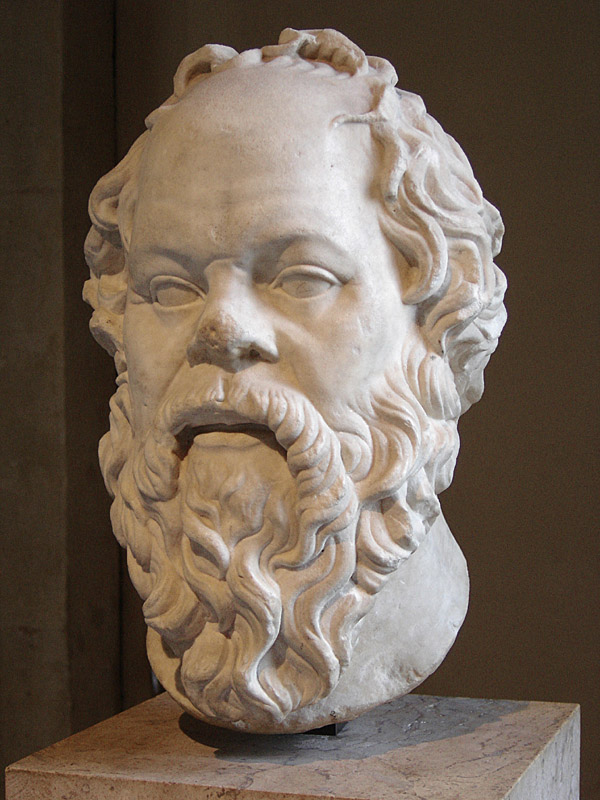
\includegraphics[width=1.0\textwidth]{figures/socrates.jpg}\\
		\centering \color{gray}{Eric Gaba (CC by-nc-sa 2.5)}
	\end{minipage}
\end{frame}

\begin{frame}{Propositional logic}
	\begin{block}{Primitives}
			Atomic values: $P, Q$\\
			Operations: $\rightarrow$\\
			Term: $P \rightarrow Q$\\
			Derivation: $H_1, \dots, H_n \vdash P$
	\end{block}

	\uncover<2->{
	\begin{block}{Proof rules}
			\begin{center}
					\begin{minipage}{.4\textwidth}
					\[
							\begin{prooftree}
									\justifies
									H, P \vdash P
									\using \text{hyp}
							\end{prooftree}
					\]
					\end{minipage}
					\begin{minipage}{.4\textwidth}
							\[
									\begin{prooftree}
											H, P \vdash Q
											\justifies
											H \vdash P \rightarrow Q
											\using \rightarrow \text{intro}
									\end{prooftree}
							\]
					\end{minipage}\\
					\vspace{1em}
					\begin{minipage}{1.0\textwidth}
					\[
							\begin{prooftree}
											H, \vdash P \rightarrow Q
											\hspace{1em}
											H \vdash P
											\justifies
											H \vdash Q
											\using \rightarrow \text{elim}_{[P]}
							\end{prooftree}
					\]
					\end{minipage}
			\end{center}
	\end{block}
	}
\end{frame}

\begin{frame}{Propositional logic \small{example}}
	\begin{block}{Theorem}
			\[ (P \rightarrow Q) \rightarrow P \rightarrow Q \]
	\end{block}
	\begin{block}{Proof}
			\[
					\begin{prooftree}
							\begin{prooftree}
									\begin{prooftree}
											\justifies
											P \rightarrow Q, \dots \vdash P \rightarrow Q
											\using \text{hyp}
									\end{prooftree}
									\hspace{1em}
									\begin{prooftree}
											\justifies
											\dots, P \vdash P
											\using \text{hyp}
									\end{prooftree}
									\justifies
									P \rightarrow Q, P \vdash Q
									\using \rightarrow \text{elim}_{[P]}
							\end{prooftree}
							\justifies
							\vdash (P \rightarrow Q) \rightarrow P \rightarrow Q
							\using \rightarrow \text{intros}
					\end{prooftree}
			\]
	\end{block}
\end{frame}

\begin{frame}{Automated Theorem Proving}
	For a (unproven) theorem, find proof consisting of these proof steps.\\
	\bigskip
	\begin{itemize}
		\item Premise selection: finding useful theorems
		\item Proof construction: applying steps
		\item Proof verification: checking correctness
	\end{itemize}
	\bigskip
	First ATP guided proof: Davis, 1957.
\end{frame}

\begin{frame}{Successes of Automated Theorem Proving}
	\begin{block}{Kepler Conjecture}
		What is the best way to stack cannonballs?
		\bigskip
		\begin{center}
				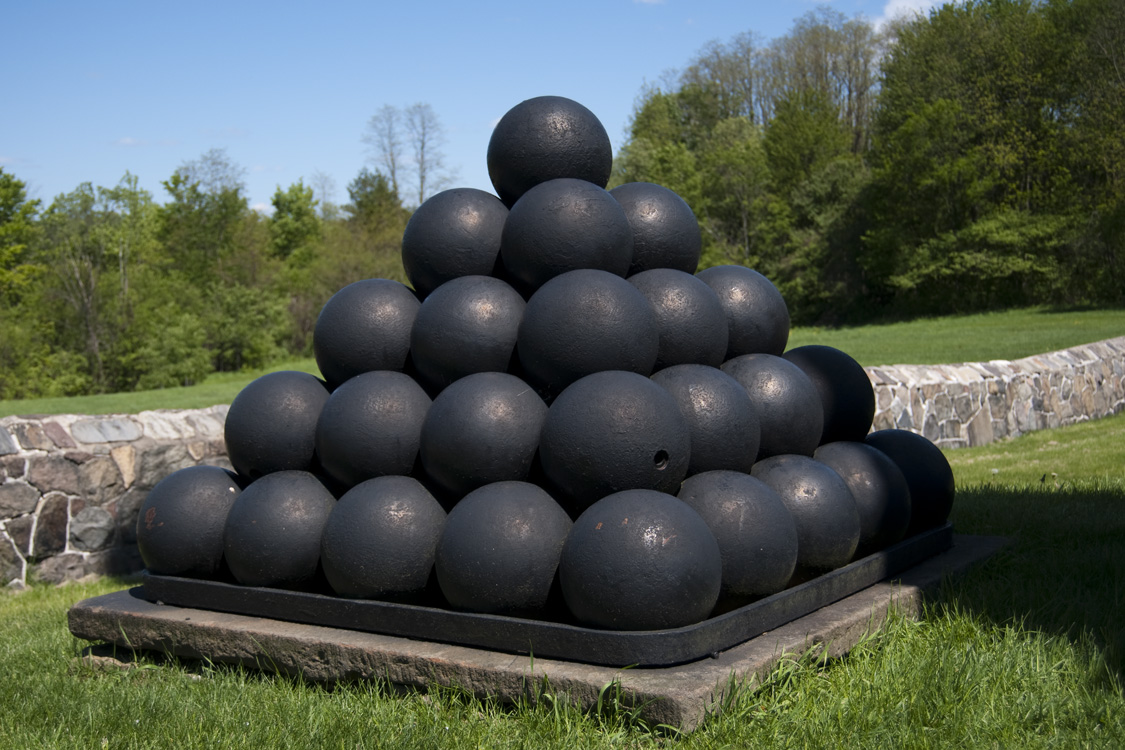
\includegraphics[width=0.5\textwidth]{figures/balls.jpg}\\
				\centering \color{gray}{Nedral (CC by-nc-sa 2.5)}
		\end{center}
		
		\small{
				No arrangement of equally sized spheres has a greater average than $\frac{\pi}{3\sqrt{2}}$.
				Formalized in 2014 by Flyspeck using Isabelle and HOL Light.
		}
	\end{block}
\end{frame}

\begin{frame}{Interactive Theorem Proving}
	\begin{center}
		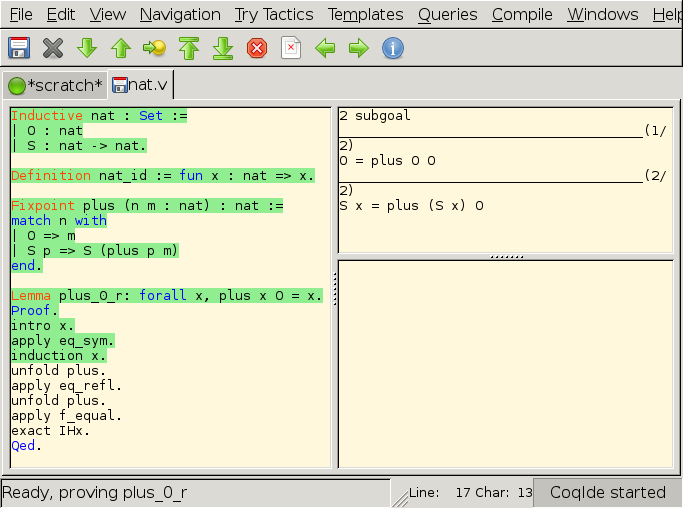
\includegraphics[height=0.78\textheight]{figures/coqide.png}
	\end{center}
\end{frame}

\begin{frame}{Premise Selection in ITP}
	\begin{center}
		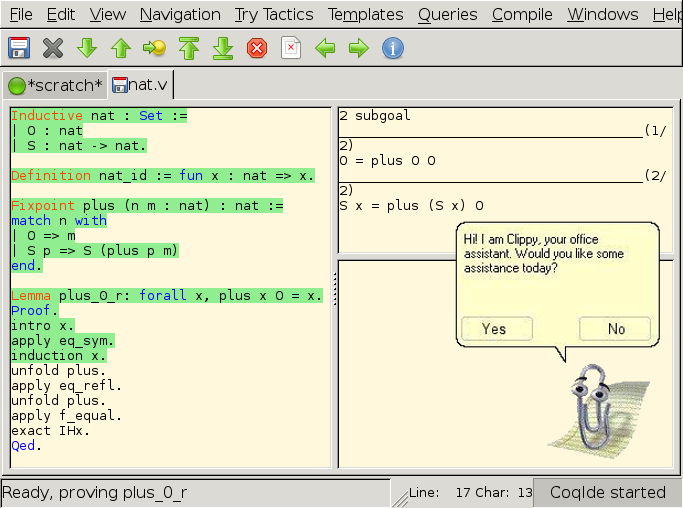
\includegraphics[height=0.78\textheight]{figures/coqide-clippy.png}
	\end{center}
\end{frame}

\begin{frame}{Source research}
	\begin{center}
		\bibentry{kaliszyk2014machine}
	\end{center}
\end{frame}

\end{document}
